\section{Theory}

\begin{frame}
        \centering
        \huge Theory
\end{frame}

\begin{frame}
	\frametitle{Diffusion Episodes}
	\begin{figure}
		\centering
		\includegraphics[scale=0.5]{diffusionepisode.png}
		\caption{Group of users before and after a diffusion episode}
	\end{figure}
	\begin{block}{Diffusion Episode Definition}
		$D = \{(\textit{u}_i, \textit{t}_i), (\textit{u}_j, \textit{t}_j)...\}$
	\end{block}
\end{frame}

\begin{frame}
	\frametitle{Representation Learning Model}
	\begin{columns}
		\begin{column}{0.6\textwidth}
			\begin{itemize}
				\item Latent space
				\begin{itemize}
					\item Latent
					\item Dimensionality Reduction
					\item Projection onto euclidean space with \textit{d} dimensions
					\item Distance correlates with chance of being the source
				\end{itemize}
				\item Receiver and Sender embeddings
			\end{itemize}
		\end{column}
		\begin{column}{0.4\textwidth}
			\begin{figure}
				\centering
				\includegraphics[scale=0.5]{latentspace.png}
			\end{figure}
		\end{column}
	\end{columns}
	\note{Latent space models were introduced by Hoff et al. (2002), and have since been
		expanded to include model-based clustering (Handcock et al., 2007) and dynamic
		networks (Sewell and Chen, 2015). Latent space models are similar to a logistic
		regression predicting whether or not a tie will occur between each pair of people in
		the network. The models include a random effect - a position in the latent space - for
		every person. The latent positions are usually constrained to lie in a low-dimensional,
		Euclidean space to make the model easier to fit and to interpret. A tie is more likely between 2 people who are closer in the latent space.}
\end{frame}

\begin{frame}
	\frametitle{Source Prediction Model}
	\begin{columns}
		\begin{column}{0.6\textwidth}
			\begin{block}{Averaged Representation of Infected Users}
				\centering
				$\textit{z}_D =
				\phi(\hat{\textit{U}}_D)=
				\frac{1}{\hat{\textit{U}}_D}
				\sum_{\textit{u}_i \in \hat{\textit{U}}_D} \textit{z}_i$
			\end{block}
			\begin{block}{Diffusion Source}
				\centering
				$s^* = argmin_{\textit{u}_i\in \textit{U}/\hat{\textit{U}_D}}
				(||\textit{w}_i - \textit{z}_D||)$
			\end{block}
		\end{column}
		\begin{column}{0.4\textwidth}
			\begin{figure}
				\centering
				\includegraphics[scale=0.5]{diffusionrepresentation.png}
			\end{figure}
		\end{column}
	\end{columns}
	\note{Making 2 latent spaces, one for receiver and one for sender\\
		Finding the source is finding the sender closest to the averaged representation of infected users
	}
\end{frame}

\begin{frame}
	\frametitle{Learning Step}
	\begin{columns}
		\begin{column}{0.45\textwidth}
			\begin{itemize}
				\item Stochastic Gradient Descent
			\end{itemize}
		\end{column}
		\begin{column}{0.4\textwidth}
			\begin{figure}
				\centering
				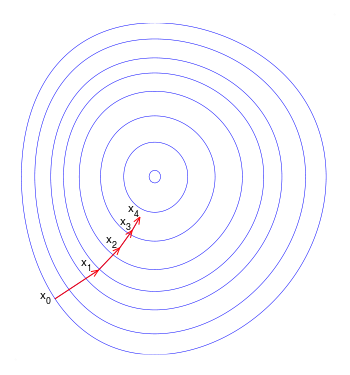
\includegraphics[scale=0.1]{gradientdescent.png}
			\end{figure}
		\end{column}
	\end{columns}
\begin{block}{Update Step}
	\centering
	$\textit{L}(\Omega, \textit{Z}) = 
	\sum_{D \in \mathcal{D}}
	\sum_{\textit{u}_i \notin \textit{U}_D}
	\textit{h}(||\textit{w}_i-\textit{z}_D||^2 - ||\textit{w}_{s_D}-\textit{z}_D||^2)
	$
\end{block}
	\begin{block}{Regularization}
		\centering
		$\textit{L}(\Omega, \textit{Z}) + \lambda \sum_{u_i}||\textit{w}_i - \textit{z}_i||^2$
	\end{block}
	\note{learning 2 embeddings Omega and Z}
\end{frame}

\begin{frame}
	\frametitle{Learning Step}
	\begin{figure}
		\centering
		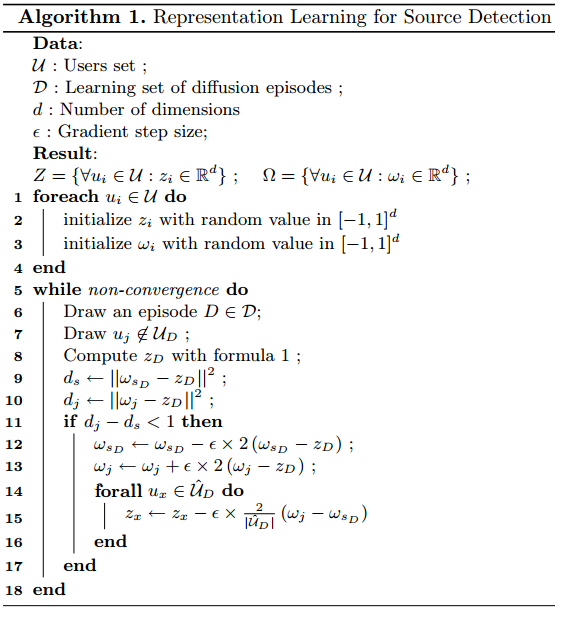
\includegraphics[scale=0.45]{Algorithm.png}
	\end{figure}
\end{frame}

\begin{frame}
	\frametitle{Extensions}
	\begin{block}{Inclusion of User Importance}
		\centering
		$z_D = \sum_{\textit{u}_i \in \hat{\textit{U}}_D}
		\frac{\textit{e}^{\alpha_i}}{
			\sum_{\textit{u}_j \in \hat{\textit{U}}_D} \textit{e}^{\alpha_j}
		} \textit{z}_i$
	\end{block}
	\begin{block}{Integration of Content}
		\centering
		$
		z_D = \frac{1}{|\hat{\textit{U}}_D|}
		\sum_{\textit{u}_i \in \hat{\textit{U}}_D} \textit{z}_i + <\textit{w}_D, \theta>
		$
	\end{block}
\end{frame}